\documentclass{beamer}

\mode<presentation>
{
  \usetheme{CambridgeUS}
  % or ...

  \setbeamercovered{transparent}
  % or whatever (possibly just delete it)
}


\usepackage[spanish]{babel}
\usepackage{graphicx}

% or whatever

\usepackage[utf8]{inputenc}
% or whatever

\usepackage{times}
\usepackage[T1]{fontenc}
% Or whatever. Note that the encoding and the font should match. If T1
% does not look nice, try deleting the line with the fontenc.

			       % packages
\title[Tucumán - Argentina] % (optional, use only with long paper titles)
{Continous laziness }

\subtitle
{``a realistic software-development new approach``} % (optional)

\author[Pablo A. Frias]           % author name, can use multiple authors (\author[author1, author2])
{
 {Pablo. A.~Frias} \textcolor{black!70}{\inst{1}\inst{2}\inst{3}}
\
}
\institute[Hack-IT  ]      % (optional, but mostly needed)
{

\textcolor{black!70}{\inst{1}}
   Hack-IT\\
   www.hack-it.com.ar
   \and
\textcolor{black!70}{\inst{2}}
   Death threats inbox\\
   pablo@hack-it.com.ar
    \and

 
\textcolor{black!70}{\inst{3}}
   Review later this talk on Github \\ 
   https://github.com/pabl0xf          
}


 \date{ \tiny Buro Coworking \\
    HackerSpace Tucuman  - 
    \textcolor{black!70}{\today}}

\subject{Talks}
% This is only inserted into the PDF information catalog. Can be left
% out. 

% If you have a file called "university-logo-filename.xxx", where xxx
% is a graphic format that can be processed by latex or pdflatex,
% resp., then you can add a logo as follows:

% \pgfdeclareimage[height=0.5cm]{university-logo}{university-logo-filename}
% \logo{\pgfuseimage{university-logo}}
                                         % presentation info - First slide


% Delete this, if you do not want the table of contents to pop up at
% the beginning of each subsection:
\AtBeginSubsection[]
{
  \begin{frame}<beamer>{Outline}
    \tableofcontents[currentsection,currentsubsection]
  \end{frame}
}


% If you wish to uncover everything in a step-wise fashion, uncomment
% the following command: 

%\beamerdefaultoverlayspecification{<+->}

\begin{document}


\begin{frame}
  \titlepage
\end{frame}


\begin{frame}{A matter of perspective}{}  
Honesty as a core value.
\begin{figure}[h]
\centering
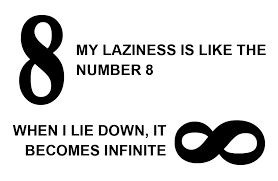
\includegraphics[scale=0.63]{../images/laziness1.png}
\end{figure}
\end{frame}


\begin{frame}{A fundamental questions}{this is how a new paradigm is born }  
\begin{figure}[h]
\centering

\includegraphics[scale=0.58]{../images/velociraptor1.jpg}
\end{figure}
\end{frame}

\begin{frame}{Project wiggle}{}  
\begin{figure}[h]
\centering

\includegraphics[scale=0.98]{../images/wiggle1.jpg}
\end{figure}
\end{frame}

\begin{frame}{Outline}
  \tableofcontents
  % You might wish to add the option [pausesections]
\end{frame}
                                 % show outline
\section{The laziness manifesto}

\subsection{First: Be awesome}



\begin{frame}{or at least pretend..}{}
  % - A title should summarize the slide in an understandable fashion
  %   for anyone how does not follow everything on the slide itself.

  \begin{itemize}
  \item
    Don't rush to broke what is already \texttt{working}.
  \pause
  \item
    Better sluggishly embrace with a stunning overfunctionality to ultimately kill what you hate. 
  \pause
\item
    When is not posible decouple to smartly extend, build over the top with a big layer of pilow  and by the end rest in the top.
  \pause
\item
    Gain confidence around and fear from the communers by doing what is aparently another level supernatural vodoo-hacker mojo while you are actually slacking off.   
  \pause
  \end{itemize}
\end{frame}


\begin{frame}{Ok, now what?}{panic attack}

\begin{figure}[h]
\centering
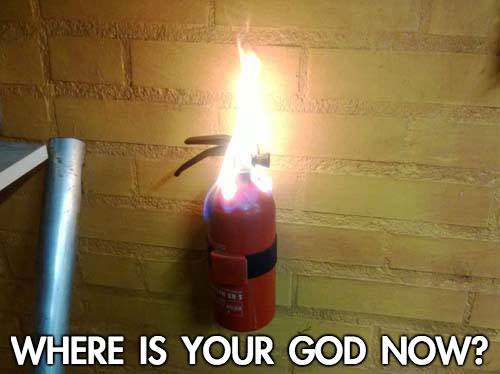
\includegraphics[scale=0.52]{../images/irony1.jpg}
\end{figure}
 
\end{frame}

\begin{frame}{Project Wingman IDE}{meant to be unseful by design}
  % - A title should summarize the slide in an understandable fashion
  %   for anyone how does not follow everything on the slide itself.

  \begin{itemize}
  \item
    I m just a filler text and I feel like I have no porpouse in life :( . \newline 
 \item
   https://github.com/pabl0xf/wingman-ide
  \item
 \pause
    Watch the demo!\newline 
  \end{itemize}
\end{frame}

\subsection{Second: Break boundaries by twisting incredulous minds}


\begin{frame}{Complexity of the absurd}{Not stupid if it works...}

\begin{itemize}
  \item
    Don't stop after \alert{automatize}  what everyone think makes sense.
  \pause
  \item
    Connect the dots where there is any dot in sight or make your own dots by force, use a gun if you need it. 
  \pause
\item
    Creativity from laziness is a bless, don't forget.
  \end{itemize}
\end{frame}

\begin{frame}{what a genious!}{ }

\begin{figure}[h]
\centering

\includegraphics[scale=0.50]{../images/stupid1.jpg}
\end{figure}
 
\end{frame}

\begin{frame}{Project coding by taking naps}{ }

\begin{itemize}
  \item
    Watch the demo !
   \end{itemize}
 
\end{frame}

\subsection{Third: Know the unspoken true}

\begin{frame}{Too lazy to complete this slide}{}

\begin{itemize}
  \item
    Nothing to see here, keep moving.
  \end{itemize}
\end{frame}


\section{The methodology in a nutshell}

\subsection{Project I would like to gain everyone hates}

\begin{frame}{Or at least half...}
  % - A title should summarize the slide in an understandable fashion
  %   for anyone how does not follow everything on the slide itself.
\begin{itemize}
 \item
   There is a meaning hide behind this, maybe.  
 \item
   https://github.com/pabl0xf/riber
  \end{itemize}
 \end{frame}

\subsection{Project talk like a pirate}
\begin{frame}{Drinking rum all day makes you a pirate }{}
\begin{figure}[h]
\centering

\includegraphics[scale=0.40]{../images/pirate1.jpg}
\end{figure}
\end{frame}

\begin{frame}{A useful plugin}{for a hackeable text-editor}
https://github.com/spudly/atom-talk-like-a-pirate
\end{frame}

 
\subsection{Project 12 monkeys}
\begin{frame}{Sorry too late, come back tomorrow}{}

 Sorry this will be part of a second talk later, if you did't have enough nosense :)  

 
\end{frame} 



                   % show conference
\section*{Conclusión}

\begin{frame}{Conclusión}

  % Keep the summary *very short*.
  \begin{itemize}
  \item
    This was a brief  \alert{talk about a new revolutionary approach in software development} the rest will be cover in propabably 10 harry-potter size books:
  \item
    \alert{sluggish software development}, as a serious alternative to the agile recent popularity   
 
    
  \end{itemize}
  
  % The following outlook is optional.
  \vskip0pt plus.5fill
  \begin{itemize}
  \item
    What is pending
    \begin{itemize}
    \item
      Twelve sad monkeys project and some security concerns
    \item
      Some crazy stuff that either was not suitable for viewers at all ages or is not compiling for some reason.  
    \end{itemize}
  \end{itemize}
\end{frame}
			% show summary
\begin{frame}{Disclaimer}
\begin{center}
All trademarks, service marks, and trade names are the property of their respective owners.
\end{center}
\end{frame}
		% show disclaimer
\begin{frame}{BSD-Like License}
\tiny
Copyright 2016 Frias Pablo A. All rights reserved.\\ \medskip
Redistribution and use in source and binary forms, with or without modification, are permitted provided that the following conditions are met:\\ \medskip
   1. Redistributions of source code must retain the above copyright notice, this list of conditions and the following disclaimer.\\
   2. Redistributions in binary form must reproduce the above copyright notice, this list of conditions and the following disclaimer in the documentation and/or other materials provided with the distribution.\\ \medskip
THIS SOFTWARE IS PROVIDED BY THE HACK-IT PROJECT ``AS IS'' AND ANY EXPRESS OR IMPLIED WARRANTIES, INCLUDING, BUT NOT LIMITED TO, THE IMPLIED WARRANTIES OF MERCHANTABILITY AND FITNESS FOR A PARTICULAR PURPOSE ARE DISCLAIMED. IN NO EVENT SHALL THE POWF PROJECT OR CONTRIBUTORS BE LIABLE FOR ANY DIRECT, INDIRECT, INCIDENTAL, SPECIAL, EXEMPLARY, OR CONSEQUENTIAL DAMAGES (INCLUDING, BUT NOT LIMITED TO, PROCUREMENT OF SUBSTITUTE GOODS OR SERVICES; LOSS OF USE, DATA, OR PROFITS; OR BUSINESS INTERRUPTION) HOWEVER CAUSED AND ON ANY THEORY OF LIABILITY, WHETHER IN CONTRACT, STRICT LIABILITY, OR TORT (INCLUDING NEGLIGENCE OR OTHERWISE) ARISING IN ANY WAY OUT OF THE USE OF THIS SOFTWARE, EVEN IF ADVISED OF THE POSSIBILITY OF SUCH DAMAGE.\\ \medskip
The views and conclusions contained in the software and documentation are those of the authors and should not be interpreted as representing official policies, either expressed or implied, of the HACK-IT Project.

\end{frame}
				% show licence

\end{document}